\documentclass[conference]{IEEEtran}
\IEEEoverridecommandlockouts
\usepackage{cite}
\usepackage{amsmath,amssymb,amsfonts}
\usepackage{algorithm}
\usepackage{algpseudocode}
\usepackage{graphicx}
\usepackage{booktabs}
\usepackage{multirow}
\usepackage{array}
\usepackage{xcolor}
\usepackage{tikz}
\usetikzlibrary{positioning,arrows.meta,fit,backgrounds,calc}
\usepackage[hyphens]{url}
\usepackage[hidelinks]{hyperref}

% ------------------------------------------------------------------
% \TBD{...}: every value or passage that depends on YOUR experiments.
% Search the compiled PDF for "TBD" and replace ALL of them before
% submission. Never replace a TBD with a number you did not measure.
% ------------------------------------------------------------------
\newcommand{\TBD}[1]{\textcolor{red}{\textbf{[TBD: #1]}}}
\newcommand{\Eloc}{E^{\mathrm{loc}}}
\newcommand{\Eacc}{E^{\mathrm{acc}}}
\newcommand{\Etraj}{E^{\mathrm{traj}}}
\newcommand{\Epool}{E^{\mathrm{pool}}}
\newcommand{\Epad}{E^{\mathrm{pad}}}
\newcommand{\ctil}{\tilde{c}}
\newcommand{\Ent}{\operatorname{Ent}}
\algrenewcommand\algorithmicrequire{\textbf{Input:}}
\algrenewcommand\algorithmicensure{\textbf{Output:}}

\begin{document}
\bstctlcite{IEEEexample:BSTcontrol}

\title{Evidence Scope and Verification Placement in Step-Level Grounding Verification for Iterative Multi-Hop Retrieval-Augmented Generation}

\author{\IEEEauthorblockN{Syed Muhammad Rayyan}
\IEEEauthorblockA{\textit{Department of Computer Science} \\
\textit{National University of Computer and Emerging Sciences (FAST-NUCES)}\\
Islamabad, Pakistan \\
i267827@isb.nu.edu.pk (corresponding author)}
}

\maketitle

\begin{abstract}
Search-interleaved large language models answer multi-hop questions by alternating reasoning steps with retrieval, and step-level grounding verifiers are increasingly used to detect intermediate claims that the retrieved evidence does not support. Existing step-level benchmarks and in-loop verifiers each fix, by convention, the evidence against which a step is judged, yet these conventions differ across studies; detection is evaluated only on naturally occurring errors in small human-labelled samples; and verification cost is not reported. We propose a controlled evaluation framework with three components: hop-localized evidence perturbation (HLEP), which removes, replaces, or counterfactually edits the gold evidence of a known hop and derives typed step labels by construction; a scope-controlled verification protocol that decouples the gold-label scope from the verifier's input scope and adds a length-matched control; and a budget-constrained verification cascade calibrated on validation data. We implement the complete pipeline for Search-R1 traces from a Qwen2.5-7B model on MuSiQue, with NLI, AlignScore, MiniCheck, and LLM-judge verifiers, evaluation by AUROC, recall at 95\% retention, and cost per question, and question-level bootstrap testing; all core components are unit-tested. As the base method, we reproduce MiniCheck-RoBERTa-L on the 29,320-pair LLM-AggreFact test set, obtaining an average balanced accuracy of 73.5\% across 11 datasets (range 57.4--88.8\%). The perturbation and evidence-scope experiments on MuSiQue are in progress. Code is available at \url{https://github.com/Rayyanz/scope-verify}.
\end{abstract}

\begin{IEEEkeywords}
retrieval-augmented generation, multi-hop question answering, step-level grounding verification, evidence perturbation, verification cost
\end{IEEEkeywords}

% ==================================================================
\section{Introduction}
% ==================================================================
Large language models (LLMs) increasingly answer knowledge-intensive questions by grounding generation in retrieved documents~\cite{lewis2020rag}. For multi-hop questions, which require chaining facts across documents~\cite{yang2018hotpotqa,ho2020twowiki,trivedi2022musique}, current systems interleave reasoning with retrieval, issuing a new search after each reasoning step~\cite{yao2023react,trivedi2023ircot,jiang2023flare,jin2025searchr1}. Each step yields an \emph{intermediate claim} that depends on the evidence retrieved so far. A claim not supported by that evidence can propagate into later steps and the final answer, a pattern documented as hallucination snowballing~\cite{zhang2024snowball}.

Two lines of work address this risk. Retrieval-control methods decide when and what to retrieve or how to correct retrieval~\cite{asai2024selfrag,yan2024crag,jeong2024adaptive}. Detection methods judge whether generated text is supported, using sampling consistency~\cite{manakul2023selfcheckgpt}, verification questions~\cite{dhuliawala2024cove}, atomic fact checking~\cite{min2023factscore}, semantic entropy~\cite{farquhar2024semantic}, trained span detectors~\cite{niu2024ragtruth}, or claim--document grounding verifiers~\cite{honovich2022true,zha2023alignscore,tang2024minicheck}. Step-level verification of intermediate reasoning is now an active area in its own right: verifiers are used inside the generation loop~\cite{zhao2023verifyedit,xu2024searchain,asai2024selfrag,kwon2026safe,kim2026prostep}, and step-level benchmarks have been released~\cite{jacovi2024reveal,ji2026stepgap,pham2026grace,chu2026locally}.

These studies share an unexamined design choice. Each fixes the evidence against which a step is judged, and the conventions differ: a paragraph retrieved per step after the fact~\cite{jacovi2024reveal}, evidence accumulated up to the step~\cite{ji2026stepgap}, the full given context with or without preceding steps~\cite{chu2026locally,kwon2026safe,pham2026grace}, or the full prefix~\cite{kim2026prostep}. To our knowledge, none varies this choice as a controlled variable, so it is unknown whether reported detection quality, or the ranking of verifiers, depends on it. In addition, existing benchmarks evaluate detection on naturally occurring errors from modest human-labelled samples (e.g., 181 steps in~\cite{ji2026stepgap}); synthetic errors and counterfactual evidence have been used to \emph{train} verifiers~\cite{kwon2026safe,chu2026locally} but not to evaluate them at a known hop. Finally, studies that compare verification granularity report detection only~\cite{jacovi2024reveal,pham2026grace}, leaving the cost of verification under iterative retrieval unmeasured.

This paper addresses three objectives: (O1) measure how step-level detection metrics and verifier rankings change across evidence scopes and gold-label definitions; (O2) estimate per-type detection under controlled evidence perturbation at a known hop; and (O3) characterize the detection--cost frontier of verification placements. The contributions are:
\begin{itemize}
\item \textbf{Hop-localized evidence perturbation (HLEP)}, a procedure that removes, replaces with an external distractor, or counterfactually edits the gold paragraph of a chosen hop, together with a formal label-construction rule that assigns typed step labels (Missing Bridge, Irrelevant Evidence, Contradicted Claim) by construction (Algorithm~\ref{alg:hlep}).
\item \textbf{A scope-controlled verification protocol} that decouples the gold-label scope from the verifier input scope, adds a length-matched control to separate scope from input length, and defines the later-supported rate as a direct measure of masking by out-of-scope evidence (Algorithm~\ref{alg:scope}).
\item \textbf{A budget-constrained verification cascade} whose escalation band is calibrated on validation data under an explicit AUROC tolerance, evaluated on a detection--cost frontier (Algorithm~\ref{alg:cascade}).
\item \textbf{A complete, unit-tested implementation} of the framework for MuSiQue with four verifiers, and a reproduction of MiniCheck~\cite{tang2024minicheck} as the base method on the full LLM-AggreFact test set; the main experiments are in progress.
\end{itemize}
The study evaluates \emph{local} step support only; question alignment and answer closure, which can fail even when every step is supported~\cite{chu2026locally}, are out of scope.

Section~\ref{sec:related} reviews related work, Section~\ref{sec:methods} describes the data, problem formulation, and methodology, Section~\ref{sec:results} reports the experiments, and Section~\ref{sec:conclusion} concludes.

% ==================================================================
\section{Related Work}\label{sec:related}
% ==================================================================
\textbf{Iterative retrieval for multi-hop reasoning.}
ReAct interleaves reasoning with tool calls~\cite{yao2023react}; IRCoT retrieves after every chain-of-thought sentence~\cite{trivedi2023ircot}; FLARE retrieves when token confidence drops~\cite{jiang2023flare}; Adaptive-RAG routes questions by predicted complexity~\cite{jeong2024adaptive}; and Search-R1 learns when and what to search with reinforcement learning~\cite{jin2025searchr1}, with a follow-up empirical study of design choices for training such reasoning--search interleaved agents~\cite{jin2025empirical}. MuSiQue was constructed to reduce the single-hop shortcuts identified in earlier multi-hop datasets~\cite{min2019compositional,trivedi2022musique}. These methods are evaluated mainly by final-answer accuracy, not by the support of each intermediate claim.

\textbf{Response-level detection and claim-level grounding.}
Consistency-based~\cite{manakul2023selfcheckgpt} and uncertainty-based~\cite{farquhar2024semantic} detectors operate on whole responses. FActScore decomposes long-form text into atomic facts~\cite{min2023factscore}, and SAFE by Wei and co-authors extends this with search~\cite{wei2024longform}; it is unrelated to the step verifier SAFE by Kwon and co-authors~\cite{kwon2026safe}. Grounding verifiers judge a claim against a document: NLI-based checkers evaluated in TRUE~\cite{honovich2022true}, AlignScore~\cite{zha2023alignscore}, and MiniCheck, which matches large-LLM accuracy on the LLM-AggreFact benchmark at far lower cost~\cite{tang2024minicheck}. These are evaluated mostly on single-turn outputs~\cite{niu2024ragtruth}.

\textbf{Step-level verification inside generation.}
Verify-and-Edit revises rationales against retrieved knowledge~\cite{zhao2023verifyedit}; SearChain verifies each node of a query chain~\cite{xu2024searchain}; Self-RAG emits segment-level relevance and support tokens~\cite{asai2024selfrag}. SAFE checks knowledge-graph-triple steps against all ten given passages plus the prefix and trains on synthetically corrupted steps~\cite{kwon2026safe}; PRO-Step is a generative process reward model scoring validity and grounding per step with the full prefix~\cite{kim2026prostep}. Process supervision was established earlier for mathematical reasoning~\cite{lightman2024verify,zheng2024processbench}. These works are evaluated by answer accuracy rather than by detection quality against reference step labels.

\textbf{Step-level grounding benchmarks.}
REVEAL labels chain-of-thought steps for attribution against evidence retrieved per step after the fact, and finds a step-level pipeline outperforms a single-decision verifier~\cite{jacovi2024reveal}. StepGap labels steps of Search-R1-style traces with typed evidence gaps under accumulated evidence, compares a hybrid NLI+LLM checker with MiniCheck and NLI, and shows that question-level F1 is inflated by checkers that flag every step~\cite{ji2026stepgap}. GRACE provides human-annotated step faithfulness labels with full context and compares all-steps-in-one-pass against step-by-step judging~\cite{pham2026grace}. Chu and co-authors adjudicate responses in a distractor setting, evaluate verifiers at response and trace level, and identify a local--global gap~\cite{chu2026locally}.

\textbf{Imperfect retrieval and knowledge conflicts.}
LLMs are distracted by irrelevant context~\cite{shi2023distracted,yoran2024robust} and sensitive to noise type and position~\cite{cuconasu2024noise}; entity substitution creates controlled conflicts between evidence and parametric knowledge~\cite{longpre2021entity}.

\begin{table*}[t]
\caption{Closest work and the variables this study manipulates.}\label{tab:related}
\centering\small
\resizebox{\textwidth}{!}{%
\begin{tabular}{@{}l l l l l l@{}}
\toprule
Work & Setting & Evidence used to judge step $t$ & Evidence perturbation & Placement / cost & Evaluated by \\
\midrule
REVEAL~\cite{jacovi2024reveal} & CoT, post-hoc evidence & One paragraph per step & No & Pipeline vs.\ single decision & Step labels \\
StepGap~\cite{ji2026stepgap} & Search-interleaved QA & Accumulated, fixed & No & No & Step F1 (181 steps) \\
Chu et al.~\cite{chu2026locally} & Distractor setting & Full context + prior steps & Training only & No & Trace AUROC, R@95 \\
SAFE~\cite{kwon2026safe} & In-loop verifier & 10 passages + prefix & No (step corruption) & No & Answer accuracy \\
GRACE~\cite{pham2026grace} & Step faithfulness & Full context & No & One pass vs.\ per step & Step F1 \\
PRO-Step~\cite{kim2026prostep} & PRM for iterative RAG & Full prefix & No & No & Answer EM/F1 \\
\textbf{This work} & Search-interleaved QA & \textbf{Varied: loc, acc, traj, pool} & \textbf{Yes, known hop} & \textbf{Detection + cost} & Step AUROC, R@95, cost \\
\bottomrule
\end{tabular}}
\end{table*}

\textbf{Synthesis.}
Table~\ref{tab:related} summarizes the positioning. Step-level verification is established both as a mechanism and as a benchmark task. What remains open is narrower: (i) whether the evidence-scope convention changes detection results and verifier rankings; (ii) per-type detection under evidence-side perturbation at a known hop; and (iii) the joint detection--cost trade-off of verification placement under iterative retrieval. These gaps motivate the framework in Section~\ref{sec:methods}.

% ==================================================================
\section{Materials and Methods}\label{sec:methods}
% ==================================================================
\subsection{Research Datasets and Data Preparation}\label{sec:data}

\textbf{MuSiQue-Ans}~\cite{trivedi2022musique} is the primary dataset. Each question has a paragraph pool of 20 Wikipedia paragraphs (gold and distractors), a gold decomposition into 2--4 single-hop sub-questions, each sub-question's answer, and the index of its supporting paragraph. These per-hop annotations are what make hop-localized perturbation and label construction possible, and the dataset was built to resist single-hop shortcuts~\cite{min2019compositional}. \textbf{2WikiMultihopQA}~\cite{ho2020twowiki} is a replication dataset with 10-paragraph contexts, evidence triples per hop, and typed questions (comparison, inference, compositional, bridge comparison). HotpotQA~\cite{yang2018hotpotqa} is used only where needed for compatibility with prior step-level label sets. Both primary datasets are publicly available from their official repositories. Table~\ref{tab:data} gives statistics; Table~\ref{tab:sample} shows the data format.

\begin{table}[t]
\caption{Dataset statistics. $^{\dagger}$Train and dev counts verified on the downloaded MuSiQue v1.0 files; other split sizes as reported in the dataset papers. Sample sizes are those used here.}\label{tab:data}
\centering\small
\resizebox{\columnwidth}{!}{%
\begin{tabular}{@{}lcc@{}}
\toprule
 & MuSiQue-Ans & 2WikiMultihopQA \\
\midrule
Train / Dev / Test & 19,938 / 2,417 / 2,459$^{\dagger}$ & 167,454 / 12,576 / 12,576 \\
Paragraphs per question & 20 & 10 \\
Hops per question & 2--4 & 2--4 \\
Per-hop gold evidence & paragraph index & evidence triple \\
\midrule
Validation sample (from train) & 100 (pilot) & 150 (planned) \\
Test sample (from dev) & 300 (preliminary) & 500 (planned) \\
\bottomrule
\end{tabular}}
\end{table}

\begin{table}[t]
\caption{Data format (constructed example in MuSiQue format, for exposition only).}\label{tab:sample}
\centering\footnotesize
\begin{tabular}{@{}p{0.22\columnwidth}p{0.70\columnwidth}@{}}
\toprule
Question & Where was the director of \emph{Inception} born? \\
Hop 1 & Who directed \emph{Inception}? $\rightarrow$ Christopher Nolan (paragraph 4) \\
Hop 2 & Where was \#1 born? $\rightarrow$ London (paragraph 11) \\
Pool & 20 paragraphs; 2 supporting, 18 distractors \\
\midrule
Trace step & ``Inception was directed by Christopher Nolan, so I need his birthplace.'' \\
Decontext.\ claim & ``\emph{Inception} was directed by Christopher Nolan.'' \\
\bottomrule
\end{tabular}
\end{table}

\textbf{Preparation.} We keep answerable questions only, and sample the test set from the development split stratified by hop count with a fixed seed; the official test labels are hidden, and dev sets are the standard evaluation choice for step-level work. A disjoint validation set is sampled from the training split and is the only data used to tune prompts, thresholds, and cascade bands. Sub-questions containing references such as ``\#1'' are resolved by substituting the gold answers of earlier hops. For 2WikiMultihopQA, each evidence triple $(s,r,o)$ defines a hop whose answer is $o$ and whose supporting paragraph is the context paragraph titled $s$.

\textbf{Step annotation.} Traces are segmented into steps, non-assertive steps (plans, questions) are filtered, and each remaining claim is decontextualized~\cite{choi2021decontext} by replacing references with their antecedents from the question and earlier steps, adding no content. Gold labels follow attribution to identified sources~\cite{rashkin2023ais}: a claim is \emph{supported} if a typical reader would conclude it from the evidence alone. Labels are produced by construction where HLEP determines them (Section~\ref{sec:hlep}) and by an LLM judge~\cite{zheng2023judge} otherwise. Human validation uses a double-annotated sample of perturbed steps; agreement is measured with Cohen's $\kappa$~\cite{cohen1960kappa} and Krippendorff's $\alpha$~\cite{krippendorff2004content}, and disagreements are adjudicated by a third annotator.

% ------------------------------------------------------------------
\subsection{Problem Formulation}\label{sec:formulation}
% ------------------------------------------------------------------
A question $q$ has a paragraph pool $P$, gold hops $h=1,\dots,H$ with sub-answers $a_h$ and supporting paragraphs $p_h^{*}\in P$. A search-interleaved generator $G$ with a retriever $\mathrm{Ret}(\cdot;P,k)$ returning the top-$k$ paragraphs produces a trajectory
\begin{equation}
\tau(q) = \big(z_1, Q_1, R_1,\, \dots,\, z_{T-1}, Q_{T-1}, R_{T-1},\, z_T, \hat{a}\big),
\end{equation}
with $R_t = \mathrm{Ret}(Q_t;P,k)$,
where $z_t$ is the reasoning text of step $t$, $Q_t$ its search query, and $\hat{a}$ the answer. Step $t$ is written \emph{after} observing $R_1,\dots,R_{t-1}$. Let $\ctil_t$ be the decontextualized claim of step $t$. We define five evidence scopes:
\begin{align}
\Eloc_t &= R_{t-1}, & \Eacc_t &= \textstyle\bigcup_{j<t} R_j, \nonumber\\
\Etraj &= \textstyle\bigcup_{j\le T} R_j, & \Epool &= P, \label{eq:scopes}\\
\Epad_t &= \Eloc_t \cup F_t, & &\text{with } |F_t \cup \Eloc_t|_{\mathrm{tok}} \approx |\Eacc_t|_{\mathrm{tok}}, \nonumber
\end{align}
where $F_t$ are filler paragraphs from other questions (irrelevant by construction), so $\Epad_t$ matches the length of $\Eacc_t$ without its content. Let $\Ent(c,E)\in\{0,1\}$ denote entailment of $c$ by evidence $E$. The gold label under gold scope $g\in\{\mathrm{acc},\mathrm{pool}\}$ is
\begin{equation}\label{eq:gold}
y_t^{(g)} = 1 - \Ent\big(\ctil_t, E_t^{g}\big),
\end{equation}
so $y=1$ denotes an \emph{ungrounded} step. The primary definition is $g=\mathrm{acc}$, i.e., the evidence available when the step was written. A verifier $v$ maps a claim and evidence to a support score $f_v(c,e)\in[0,1]$. For input scope $\sigma\in\{\mathrm{loc},\mathrm{acc},\mathrm{traj},\mathrm{pool},\mathrm{pad}\}$, the step score aggregates over chunks of the evidence:
\begin{equation}\label{eq:score}
s_{v,\sigma}(t) = \max_{e\,\in\,\mathrm{chunk}(E_t^{\sigma})} f_v(\ctil_t, e),
\qquad \hat{y}_t = \mathbf{1}\big[s_{v,\sigma}(t) < \theta_v\big].
\end{equation}

\textbf{Task.} Given traces, labels $y^{(g)}$, and verifiers $\{f_v\}$, estimate detection quality $D(v,\sigma,g,m)$ for every verifier, input scope, gold scope, and evidence condition $m\in\{\mathrm{clean},\mathrm{rem},\mathrm{dis},\mathrm{cf}\}$, and cost $C(v,\pi)$ for each placement $\pi$. The research questions map to these quantities: RQ1 (Gap 1) asks how $D$ varies with $\sigma$ and $g$, and whether the ranking of verifiers by $D$ changes with $\sigma$; RQ2 (Gap 2) asks how $D$ varies with $m$ and whether the scope effect interacts with $m$; RQ3 (Gap 3) asks which placements are Pareto-efficient in $(C, D)$.

\textbf{Hypotheses.} H1a: under $g=\mathrm{acc}$, recall at 95\% retention is lower with $\sigma\in\{\mathrm{traj},\mathrm{pool}\}$ than with $\sigma=\mathrm{acc}$ (masking). H1b: at least one verifier pair reverses AUROC order between scopes. H1c: estimates differ between $g=\mathrm{acc}$ and $g=\mathrm{pool}$. H2a: recall differs across perturbation types. H2b: the masking effect differs across types. H3: a cascade is non-inferior to exhaustive LLM-judge verification within margin $\delta$ at lower cost. Each has the corresponding null of no difference (or inferiority for H3).

\textbf{Assumptions and constraints.} Generation is deterministic (temperature 0); verifiers are used off the shelf without fine-tuning; the retrieval corpus for each question is its own pool, making perturbation exact; and only local support is assessed.

% ------------------------------------------------------------------
\subsection{Proposed Methodology}\label{sec:method}
% ------------------------------------------------------------------
\begin{figure*}[t]
\centering
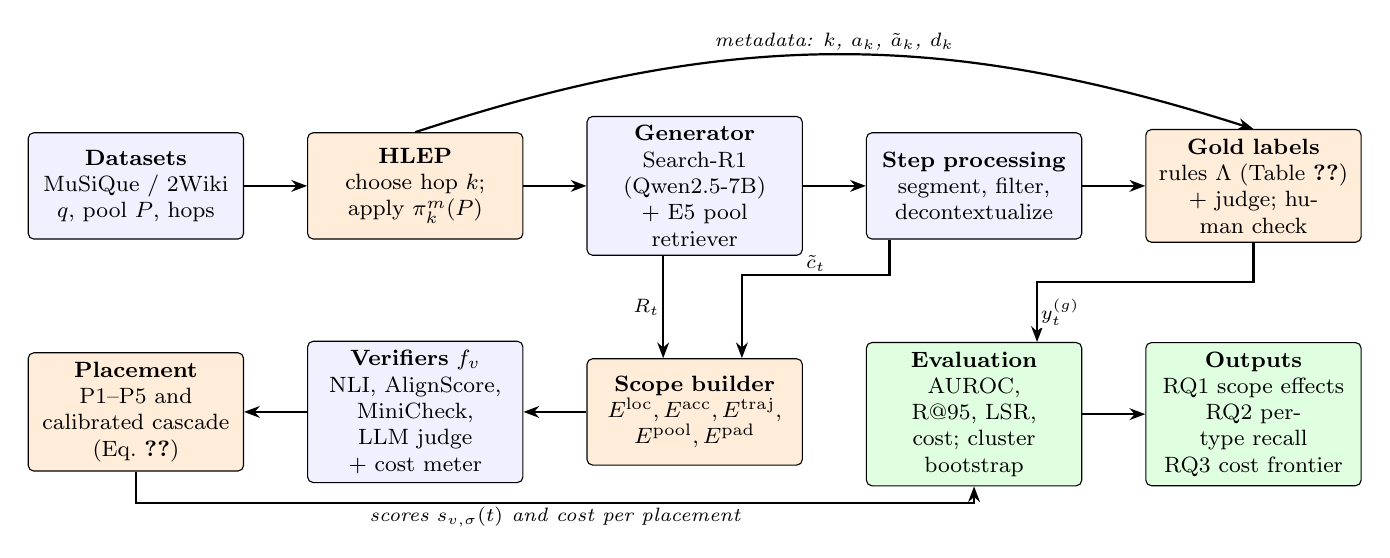
\begin{tikzpicture}[
  node distance=0.6cm and 0.8cm,
  box/.style={draw, rounded corners=2pt, align=center, font=\footnotesize, minimum height=1.35cm, text width=2.5cm, fill=#1},
  box/.default={white},
  arr/.style={-{Stealth[length=2mm]}, thick},
  lab/.style={font=\scriptsize\itshape, align=center, fill=white, inner sep=1pt}
]
% row 1
\node[box=blue!6] (data) {\textbf{Datasets}\\MuSiQue / 2Wiki\\$q$, pool $P$, hops};
\node[box=orange!15, right=of data] (hlep) {\textbf{HLEP}\\choose hop $k$;\\apply $\pi^{m}_k(P)$};
\node[box=blue!6, right=of hlep] (gen) {\textbf{Generator}\\Search-R1 (Qwen2.5-7B)\\+ E5 pool retriever};
\node[box=blue!6, right=of gen] (seg) {\textbf{Step processing}\\segment, filter,\\decontextualize};
\node[box=orange!15, right=of seg] (lab) {\textbf{Gold labels}\\rules $\Lambda$ (Table~\ref{tab:rules})\\+ judge; human check};
% row 2
\node[box=orange!15, below=1.3cm of gen] (scope) {\textbf{Scope builder}\\$\Eloc,\Eacc,\Etraj,$\\$\Epool,\Epad$};
\node[box=blue!6, left=of scope] (ver) {\textbf{Verifiers} $f_v$\\NLI, AlignScore,\\MiniCheck, LLM judge\\+ cost meter};
\node[box=orange!15, left=of ver] (casc) {\textbf{Placement}\\P1--P5 and\\calibrated cascade\\(Eq.~\ref{eq:band})};
\node[box=green!12, below=1.3cm of seg] (eval) {\textbf{Evaluation}\\AUROC, R@95, LSR,\\cost; cluster\\bootstrap};
\node[box=green!12, right=of eval] (out) {\textbf{Outputs}\\RQ1 scope effects\\RQ2 per-type recall\\RQ3 cost frontier};
% arrows row 1
\draw[arr] (data) -- (hlep);
\draw[arr] (hlep) -- (gen);
\draw[arr] (gen) -- (seg);
\draw[arr] (seg) -- (lab);
\draw[arr] (hlep.north) to[bend left=18] node[lab, above]{metadata: $k$, $a_k$, $\tilde a_k$, $d_k$} (lab.north);
% down
\draw[arr] ([xshift=-4mm]gen.south) -- node[lab, left]{$R_t$} ([xshift=-4mm]scope.north);
\draw[arr] (seg.south west) ++(3mm,0) |- ++(0,-0.45) -| ([xshift=6mm]scope.north) node[lab, pos=0.25, above]{$\ctil_t$};
% row 2
\draw[arr] (scope) -- (ver);
\draw[arr] (ver) -- (casc);
\draw[arr] (casc.south) -- ++(0,-0.4) -| node[lab, pos=0.25, below]{scores $s_{v,\sigma}(t)$ and cost per placement} (eval.south);
\draw[arr] (lab.south) |- ++(0,-0.5) -| node[lab, pos=0.75, right]{$y_t^{(g)}$} ([xshift=8mm]eval.north);
\draw[arr] (eval) -- (out);
\end{tikzpicture}
\caption{Workflow of the proposed evaluation framework. Orange components are introduced in this work; blue components are existing models used without modification; green components compute metrics and statistics.}\label{fig:workflow}
\end{figure*}

\textbf{Overview.} Fig.~\ref{fig:workflow} shows the framework. HLEP perturbs the gold evidence of one hop per question; the generator produces traces over the (possibly perturbed) pool; steps are segmented and decontextualized; gold labels are constructed; the scope builder assembles each step's evidence under every scope; each verifier scores every (claim, scope) pair while a cost meter records tokens, model calls, and GPU time; placement configurations, including a calibrated cascade, are derived from these scores; and the evaluation module computes metrics with question-level bootstrap intervals. No component is trained: the framework's contribution is the controlled perturbation, the scope protocol, and the calibrated cascade, which together turn existing verifiers into objects of controlled measurement.

\textbf{Model architecture and components.}
The generator is the released Search-R1 checkpoint \nolinkurl{PeterJinGo/SearchR1-nq_hotpotqa_train-qwen2.5-7b-em-ppo}~\cite{jin2025searchr1}, obtained by PPO training of base Qwen2.5-7B~\cite{qwen2024qwen25} on NQ and HotpotQA with an exact-match reward; MuSiQue and 2WikiMultihopQA are therefore outside its training data. It is served with vLLM~\cite{kwon2023vllm} and emits reasoning in \texttt{<think>} tags, queries in \texttt{<search>} tags, receives results in \texttt{<information>} tags, and ends with \texttt{<answer>}. The prompt, the format of the returned results, three passages per search, and a limit of four searches follow the official Search-R1 code. Retrieval uses E5~\cite{wang2022e5} embeddings via Sentence-Transformers~\cite{reimers2019sbert} with cosine similarity over the question's pool. The verifiers are a DeBERTa-v3-large NLI cross-encoder~\cite{he2023debertav3,honovich2022true} whose score is the entailment probability; AlignScore~\cite{zha2023alignscore}; MiniCheck~\cite{tang2024minicheck}; and an LLM judge (Mistral-7B-Instruct-v0.3), from a different model family than the generator, prompted with the annotation rule and scored by the normalized probability of the \textsc{Supported} option. Labels are produced by a separate judge (Llama-3.1-8B-Instruct), which is never evaluated as a verifier.

\subsubsection{Hop-localized evidence perturbation (HLEP)}\label{sec:hlep}
For each question, a hop $k$ is chosen (by default a non-final hop, whose answer is a bridge entity used by later hops). Let $D$ be the set of paragraphs from \emph{other} questions' pools, and $\bar{q}_k$ the resolved sub-question. The three perturbation operators are
\begin{align}
\pi^{\mathrm{rem}}_k(P) &= P\setminus\{p_k^{*}\}, \nonumber\\
\pi^{\mathrm{dis}}_k(P) &= \big(P\setminus\{p_k^{*}\}\big)\cup\{d_k\}, \label{eq:perturb}\\
\pi^{\mathrm{cf}}_k(P) &= \big(P\setminus\{p_k^{*}\}\big)\cup\{\tilde{p}_k\}, \nonumber
\end{align}
with
\begin{equation}
d_k=\operatorname*{arg\,max}_{p\in D,\;a_k\notin p}\mathrm{sim}(\bar{q}_k,p),\qquad \tilde{p}_k=p_k^{*}[a_k\mapsto\tilde{a}_k],
\end{equation}
and $\tilde{a}_k\sim\mathcal{S}(\mathrm{type}(a_k))\setminus\{a_k\}$,
where $p[a\mapsto b]$ replaces every occurrence of $a$ in $p$ (title and text) with $b$, and $\mathcal{S}(\cdot)$ is the set of answers of the same type (year, number, or named entity) drawn from other questions, following entity-substitution counterfactuals~\cite{longpre2021entity}. Drawing the distractor from outside the pool is necessary: replacing $p_k^{*}$ with a paragraph already in $P$ would reduce $\pi^{\mathrm{dis}}$ to $\pi^{\mathrm{rem}}$.

A step is \emph{aligned} to hop $k$ if its claim mentions $a_k$ or $\tilde{a}_k$ after normalization. Writing $\mathrm{has}(c,a)$ for normalized containment of $a$ in claim $c$ and $\mathrm{in}(E,a)$ for its containment in any paragraph of $E$, the label of an aligned step under condition $m$ is
\begin{equation}\label{eq:label}
\ell_t=\Lambda(m,\mathbf{x}_t),
\end{equation}
where $\mathbf{x}_t=\big(\mathrm{has}(\ctil_t,a_k),\,\mathrm{has}(\ctil_t,\tilde{a}_k),\,\mathrm{in}(\Eacc_t,a_k),\,[d_k\!\in\!\Eacc_t],\,[\tilde{p}_k\!\in\!\Eacc_t]\big)$ and the rule table $\Lambda$ is given in Table~\ref{tab:rules},

\begin{table}[t]
\caption{Label-construction rules $\Lambda$ of Eq.~\eqref{eq:label} for a step aligned to hop $k$. Any case not listed returns $\bot$ (labelled by the judge).}\label{tab:rules}
\centering\footnotesize
\begin{tabular}{@{}lp{0.52\columnwidth}l@{}}
\toprule
Condition & Requirements on step $t$ & Label \\
\midrule
rem, dis & states $a_k$; $\neg\mathrm{in}(\Eacc_t,a_k)$; $d_k\notin\Eacc_t$ & \textsc{MB} \\
dis & states $a_k$; $\neg\mathrm{in}(\Eacc_t,a_k)$; $d_k\in\Eacc_t$ & \textsc{IE} \\
cf & states $a_k$, not $\tilde{a}_k$; $\tilde{p}_k\in\Eacc_t$; $\neg\mathrm{in}(\Eacc_t,a_k)$ & \textsc{CC} \\
cf & states $\tilde{a}_k$; $\tilde{p}_k\in\Eacc_t$ & \textsc{Sup} \\
\bottomrule
\end{tabular}
\end{table}
\noindent where \textsc{MB}, \textsc{IE}, and \textsc{CC} are the Missing Bridge, Irrelevant Evidence, and Contradicted Claim types of~\cite{ji2026stepgap}, and $\bot$ defers to the judge. The containment checks prevent a false \emph{ungrounded} label when another paragraph also states $a_k$. In the counterfactual condition, an aligned claim stating $\tilde{a}_k$ is \emph{supported} by the evidence even though it is factually false, which separates grounding from factuality and directly exposes reliance on parametric knowledge~\cite{longpre2021entity,sainz2023contamination}.

\begin{algorithm}[t]
\caption{HLEP perturbation and label construction}\label{alg:hlep}
\begin{algorithmic}[1]
\Require question $q$ with pool $P$, hops $\{(\bar{q}_h,a_h,p_h^{*})\}$; external pool $D$; condition $m$; seed
\Ensure perturbed pool $P'$; labelled steps
\State $k \gets$ \Call{ChooseHop}{$H$, seed} \Comment{non-final hop by default}
\If{$m=\mathrm{rem}$} $P' \gets P\setminus\{p_k^{*}\}$
\ElsIf{$m=\mathrm{dis}$} compute $d_k$ (Eq.~\ref{eq:perturb})
\State $P' \gets (P\setminus\{p_k^{*}\})\cup\{d_k\}$
\ElsIf{$m=\mathrm{cf}$} draw $\tilde{a}_k$; $\tilde{p}_k \gets p_k^{*}[a_k\mapsto\tilde{a}_k]$
\State $P' \gets (P\setminus\{p_k^{*}\})\cup\{\tilde{p}_k\}$
\Else\ $P'\gets P$
\EndIf
\State \textbf{assert} perturbation applied (e.g., $a_k\notin\tilde{p}_k$)
\State $\tau \gets G(q, \mathrm{Ret}(\cdot;P',k))$
\State $\{\ctil_t\} \gets$ \Call{SegmentDecontext}{$\tau$}
\For{each step $t$}
  \If{$m\neq\mathrm{clean}$ \textbf{and} step $t$ aligned to hop $k$} $\ell_t \gets$ Eq.~\eqref{eq:label}
  \Else\ $\ell_t \gets \bot$
  \EndIf
  \If{$\ell_t=\bot$} $\ell_t \gets$ \Call{Judge}{$\ctil_t$, $\Eacc_t$}
  \EndIf
\EndFor
\State \Return $P'$, $\{(\ctil_t,\ell_t)\}$
\end{algorithmic}
\end{algorithm}

\subsubsection{Scope-controlled verification}
For every step and every scope in Eq.~\eqref{eq:scopes}, each verifier produces $s_{v,\sigma}(t)$ via Eq.~\eqref{eq:score}. Chunks are single paragraphs for encoder verifiers (whose inputs are limited to 512 tokens) and the full scope for the LLM judge; the aggregation rule is fixed across scopes so that differences are attributable to evidence content rather than to processing. The padded scope $\Epad$ isolates input length: if detection with $\Epad$ matches $\Eloc$ but differs from $\Eacc$, the scope effect is due to content, not length. Masking by later evidence is measured by the later-supported rate,
\begin{equation}\label{eq:lsr}
\mathrm{LSR} = \frac{\big|\{t:\ y_t^{(\mathrm{acc})}=1,\ \Ent(\ctil_t,\Etraj)=1\}\big|}{\big|\{t:\ y_t^{(\mathrm{acc})}=1\}\big|},
\end{equation}
the fraction of steps that were ungrounded when written but are entailed by evidence retrieved later. A verifier given $\Etraj$ or $\Epool$ can only detect such steps by error, so LSR bounds the recall loss predicted by H1a.

\begin{algorithm}[t]
\caption{Scope-controlled scoring with cost metering}\label{alg:scope}
\begin{algorithmic}[1]
\Require labelled steps; verifiers $\mathcal{V}$; scopes $\Sigma$; gold scopes $\{\mathrm{acc},\mathrm{pool}\}$
\Ensure score table $\mathcal{T}$ with rows $(q,t,v,\sigma,s,\text{tokens},\text{calls},\text{sec})$
\For{each question $q$, step $t$}
  \State build $E_t^{\sigma}$ for all $\sigma\in\Sigma$ (Eq.~\ref{eq:scopes})
  \For{each $v\in\mathcal{V}$, $\sigma\in\Sigma$}
    \State start meter; $s \gets \max_{e\in\mathrm{chunk}(E_t^\sigma)} f_v(\ctil_t,e)$; stop meter
    \State append $(q,t,v,\sigma,s,\text{cost})$ to $\mathcal{T}$
  \EndFor
\EndFor
\State join $\mathcal{T}$ with $y^{(\mathrm{acc})}, y^{(\mathrm{pool})}$; \Return $\mathcal{T}$
\end{algorithmic}
\end{algorithm}

\subsubsection{Verification placements and calibrated cascade}
Five placements are compared. P1: every step verified by the LLM judge. P2: every step verified by a non-LLM verifier. P3: a cascade in which a cheap verifier $c$ scores every step and steps whose score falls in an uncertainty band $[\ell,u]$ are escalated to the judge $J$. P4: one judge call over all steps of a trace, following~\cite{pham2026grace}. P5: response-level decomposition~\cite{min2023factscore} of the final rationale and answer, with each atomic claim mapped back to the step of maximal lexical overlap. For detection alone, verifying a step during generation or afterwards is equivalent when the unit and evidence are identical; placement is therefore defined by unit and batching, not timing. The cascade score and per-question cost are
\begin{equation}
s^{\mathrm{casc}}_t=\begin{cases}f_J(\ctil_t,E_t) & \text{if } \ell\le f_c(\ctil_t,E_t)\le u,\\ f_c(\ctil_t,E_t) & \text{otherwise,}\end{cases}
\end{equation}
\begin{equation}
C^{\mathrm{casc}}=\textstyle\sum_t\big(\kappa_c+\mathbf{1}[\ell\le f_c(\ctil_t,E_t)\le u]\,\kappa_J\big),
\end{equation}
where $\kappa_c,\kappa_J$ are the measured per-step costs. Following cost-aware LLM cascades~\cite{chen2023frugalgpt}, the band is chosen on validation data by
\begin{equation}\label{eq:band}
\begin{split}
(\ell^{*},u^{*})=\;&\operatorname*{arg\,min}_{\ell\le u}\ \mathbb{E}\big[C^{\mathrm{casc}}\big]\\
&\text{s.t. } \mathrm{AUROC}(s^{\mathrm{casc}})\ge\mathrm{AUROC}(f_J)-\delta,
\end{split}
\end{equation}
with $\delta$ fixed before test evaluation.

\begin{algorithm}[t]
\caption{Cascade band calibration}\label{alg:cascade}
\begin{algorithmic}[1]
\Require validation scores $f_c$, $f_J$, labels $y$; costs $\kappa_c,\kappa_J$; tolerance $\delta$; grid $\Lambda$
\Ensure band $(\ell^{*},u^{*})$
\State $A_J\gets\mathrm{AUROC}(f_J,y)$; best $\gets(\varnothing,\infty)$
\For{$(\ell,u)\in\Lambda$ with $\ell\le u$}
  \State compute $s^{\mathrm{casc}}$ and $\bar{C}=\kappa_c+\kappa_J\cdot\Pr[\ell\le f_c\le u]$
  \If{$\mathrm{AUROC}(s^{\mathrm{casc}},y)\ge A_J-\delta$ \textbf{and} $\bar{C}<$ best.cost} best $\gets((\ell,u),\bar{C})$
  \EndIf
\EndFor
\State \Return best band (or ``no feasible band'')
\end{algorithmic}
\end{algorithm}

\textbf{Training and optimization.} No model parameters are trained or fine-tuned. The only fitted quantities are each verifier's decision threshold $\theta_v$, chosen to maximize step F1 on the validation set, and the cascade band of Eq.~\eqref{eq:band}, chosen by grid search over $\Lambda=\{0,0.05,\dots,1\}^2$. Fitting these on validation data only prevents optimistic bias on the test set.

\textbf{Inference and execution.} For a new question, the pipeline (i) applies the chosen condition to the pool, (ii) runs the generator to completion at temperature 0 with at most $T_{\max}$ search turns, (iii) segments and decontextualizes the steps, (iv) assigns labels, (v) builds all scopes and scores every (claim, scope, verifier) triple while metering cost, and (vi) derives placement scores. All outputs are stored as JSONL keyed by question and step identifiers so that every metric is recomputable.

\textbf{Technical novelty and justification.} Table~\ref{tab:novelty} maps each gap to the mechanism that addresses it. The framework does not propose a new verifier; its novelty is in measurement. HLEP is, to our knowledge, the first use of evidence-side perturbation at a known hop to \emph{evaluate} step-level verifiers, whereas prior work used step corruption or counterfactuals for training~\cite{kwon2026safe,chu2026locally}. The scope protocol differs from prior benchmarks, which each fix one convention~\cite{jacovi2024reveal,ji2026stepgap,pham2026grace,chu2026locally}, by treating scope as a controlled variable, separating it from length, and quantifying masking (LSR). The calibrated cascade adapts cost-aware cascading~\cite{chen2023frugalgpt} to step-level grounding with an explicit detection tolerance, which prior granularity comparisons~\cite{jacovi2024reveal,pham2026grace} do not report.

\begin{table}[t]
\caption{Mapping of gaps to mechanisms and evidence.}\label{tab:novelty}
\centering\footnotesize
\begin{tabular}{@{}p{0.27\columnwidth}p{0.33\columnwidth}p{0.28\columnwidth}@{}}
\toprule
Gap & Mechanism & Evaluated by \\
\midrule
G1: scope is a fixed, differing convention & Scope protocol, Eqs.~\eqref{eq:scopes}--\eqref{eq:score}, LSR Eq.~\eqref{eq:lsr} & RQ1; H1a--H1c \\
G2: no evidence-side perturbation for evaluation & HLEP, Eqs.~\eqref{eq:perturb}--\eqref{eq:label}, Alg.~\ref{alg:hlep} & RQ2; H2a--H2b \\
G3: detection--cost trade-off unmeasured & Calibrated cascade, Eq.~\eqref{eq:band}, Alg.~\ref{alg:cascade} & RQ3; H3 \\
\bottomrule
\end{tabular}
\end{table}

% ==================================================================
\section{Experimental Results and Discussion}\label{sec:results}
% ==================================================================
\subsection{Experimental Setup and Implementation}
\textbf{Environment.} Experiments run on Kaggle notebooks with two NVIDIA Tesla T4 GPUs (16\,GB each); LLMs run in fp16 with tensor parallelism over both GPUs, since the T4 does not support bfloat16. The software stack is Python 3.13, PyTorch 2.14.0 (CUDA 13.0), Hugging Face Transformers 5.20.2, vLLM~\cite{kwon2023vllm} 0.33.0, and Sentence-Transformers~\cite{reimers2019sbert}. Table~\ref{tab:config} lists the configuration.

\begin{table}[t]
\caption{Configuration of implemented components.}\label{tab:config}
\centering\footnotesize
\resizebox{\columnwidth}{!}{%
\begin{tabular}{@{}ll@{}}
\toprule
Component & Setting \\
\midrule
Generator & \texttt{PeterJinGo/SearchR1-nq\_hotpotqa\_train-qwen2.5-7b-em-ppo} \\
Decoding & greedy (temperature 0); 512 new tokens per turn; at most 4 searches \\
Precision & fp16; vLLM tensor parallel size 2; max length 8,192 tokens \\
Retriever & \texttt{intfloat/e5-base-v2}; top-$k=3$; per-question pool \\
NLI verifier & \texttt{MoritzLaurer/DeBERTa-v3-large-mnli-fever-anli-ling-wanli} \\
AlignScore & RoBERTa-large, \texttt{nli\_sp} mode \\
MiniCheck & \texttt{roberta-large} checkpoint (MiniCheck-RoBERTa-L) \\
LLM judge & \texttt{mistralai/Mistral-7B-Instruct-v0.3}; 3-way prompt; score $=P(\textsc{Sup})$ \\
Label judge & \texttt{meta-llama/Llama-3.1-8B-Instruct} \\
Thresholds & max step F1 on validation \\
Cascade & grid step 0.05; $\delta$ fixed after the pilot, before test evaluation \\
Bootstrap & $B=10{,}000$ question-level resamples; seed 13 \\
\bottomrule
\end{tabular}}
\end{table}

\textbf{Implementation status.} Table~\ref{tab:status} lists every component of the workflow in Fig.~\ref{fig:workflow}, the module that implements it, and its status. All components are implemented in Python as a single package. The core logic is covered by unit tests: HLEP operators (removal, external distractor, counterfactual substitution with same-type substitutes that never coincide with another answer of the same question), the label-construction rules of Table~\ref{tab:rules}, the evidence scopes of Eq.~\eqref{eq:scopes} including the length-matched control, the metrics of Table~\ref{tab:metrics}, the cluster bootstrap with Holm correction, and cascade band calibration; all nine tests pass. The tests exposed and fixed one design flaw: without type matching and exclusion, a counterfactual substitute for a person could be a place that is the answer to another hop of the same question. The analysis script was additionally run end to end on synthetic score tables to verify the statistics pipeline; no results from synthetic data are reported.

\begin{table}[t]
\caption{Implementation status of the workflow components.}\label{tab:status}
\centering\footnotesize
\resizebox{\columnwidth}{!}{%
\begin{tabular}{@{}lll@{}}
\toprule
Component & Module & Status \\
\midrule
Data loading, stratified sampling & \texttt{data.py} & implemented; data downloaded \\
Per-question E5 retriever & \texttt{retriever.py} & implemented \\
HLEP perturbation (Eqs.~\ref{eq:perturb}) & \texttt{perturb.py} & implemented, tested \\
Search-R1 trace generation & \texttt{generate.py} & implemented; run pending \\
Step segmentation, decontextualization & \texttt{claims.py} & implemented \\
Label construction (Table~\ref{tab:rules}) & \texttt{labels.py} & implemented, tested \\
Evidence scopes (Eq.~\ref{eq:scopes}) & \texttt{scopes.py} & implemented, tested \\
Verifiers + cost meter (Eq.~\ref{eq:score}) & \texttt{verifiers.py} & implemented \\
Calibrated cascade (Alg.~\ref{alg:cascade}) & \texttt{cascade.py} & implemented, tested \\
Metrics, bootstrap, Holm & \texttt{metrics.py}, \texttt{stats.py} & implemented, tested \\
Base reproduction (MiniCheck) & \texttt{reproduce\_minicheck.py} & \textbf{executed} (Table~\ref{tab:repro}) \\
\bottomrule
\end{tabular}}
\end{table}

\textbf{Reproducibility.} Generation is greedy; all random choices (sampling, hop choice, substitutes, bootstrap) use fixed seeds; model identifiers are fixed in a single configuration file; and intermediate outputs (pools, traces, labels, score tables) are written as JSONL or CSV keyed by question and step identifiers, so every metric can be recomputed.

\subsection{Evaluation Metrics}
The positive class is \emph{ungrounded}. Table~\ref{tab:metrics} defines the metrics. AUROC is threshold-free and is the primary ranking metric, as in prior hallucination-detection work~\cite{farquhar2024semantic,manakul2023selfcheckgpt}; recall at 95\% retention follows~\cite{chu2026locally}; step F1 and balanced accuracy allow comparison with step-level benchmarks~\cite{ji2026stepgap,pham2026grace} and LLM-AggreFact~\cite{tang2024minicheck}. Balanced accuracy is used across conditions because the base rate of ungrounded steps differs by condition. Question-level F1 is reported only next to a flag-all baseline, because it is inflated by checkers that flag every step~\cite{ji2026stepgap}.

\begin{table*}[t]
\caption{Evaluation metrics. $s$: support score; $y=1$: ungrounded; $\theta$: threshold; $\mathcal{U},\mathcal{S}$: ungrounded and supported steps.}\label{tab:metrics}
\centering\footnotesize
\begin{tabular}{@{}p{3.0cm}p{7.6cm}p{5.6cm}@{}}
\toprule
Metric & Definition & Purpose \\
\midrule
AUROC & $\Pr\big[s_i<s_j \mid i\in\mathcal{U}, j\in\mathcal{S}\big]$ & Threshold-free ranking; RQ1--RQ3 \\
Recall at 95\% retention (R@95) & $\theta_{95}=\sup\{\theta:\Pr[s\ge\theta\mid\mathcal{S}]\ge0.95\}$;\ \ R@95$=\Pr[s<\theta_{95}\mid\mathcal{U}]$ & Errors caught at a fixed 5\% false-alarm rate; H1a, H2a \\
Step F1 & $2PR/(P+R)$ at validation-tuned $\theta$ & Comparability with~\cite{ji2026stepgap,pham2026grace} \\
Balanced accuracy & $\tfrac12\big(\tfrac{TP}{TP+FN}+\tfrac{TN}{TN+FP}\big)$ & Robust to base-rate differences; base reproduction \\
AUPRC & area under precision--recall curve (with base rate) & Within-condition only \\
LSR & Eq.~\eqref{eq:lsr} & Masking mechanism; H1a \\
Rank reversal & pair $(v,v')$ with $\Delta\mathrm{AUROC}$ of opposite sign and 95\% CIs excluding 0 in two scopes & H1b \\
Cost & tokens, model calls, verifier passes, GPU-seconds per question & RQ3, H3 \\
Label agreement & Cohen's $\kappa$~\cite{cohen1960kappa}; Krippendorff's $\alpha$~\cite{krippendorff2004content} & Validity of labels \\
\bottomrule
\end{tabular}
\end{table*}

\textbf{Statistical analysis.} Steps are nested in questions, so confidence intervals use a cluster bootstrap that resamples questions with replacement~\cite{efron1993bootstrap,koehn2004significance,dror2018hitchhiker}. For a statistic $\Delta$ (e.g., an AUROC difference between two scopes), the $b$-th replicate is computed on the steps of a resampled question set $\mathcal{Q}^{(b)}$, and the 95\% interval is $[\Delta^{(2.5)},\Delta^{(97.5)}]$ over $B=10{,}000$ replicates. The six primary tests are corrected with the Holm procedure~\cite{holm1979simple}. H3 is tested for non-inferiority: the lower bound of the interval for $\mathrm{AUROC}(\mathrm{P3})-\mathrm{AUROC}(\mathrm{P1})$ must exceed $-\delta$.

\subsection{Baseline Implementation and Reproduction}
\textbf{Base paper.} The principal reproduced method is MiniCheck~\cite{tang2024minicheck}, a grounding verifier that is also one of the evaluated verifiers and the strongest low-cost baseline used in step-level work~\cite{ji2026stepgap}. We reproduce MiniCheck-RoBERTa-L on all 11 datasets of the LLM-AggreFact test set (29,320 claim--document pairs) with the released checkpoint and the authors' evaluation protocol: scores are converted to labels at a threshold of 0.5, balanced accuracy is computed per dataset, and the unweighted mean is reported. Table~\ref{tab:repro} shows the results, together with the published leaderboard values of the larger MiniCheck-Flan-T5-L~\cite{llmaggrefact2026leaderboard} for context.

\begin{table}[t]
\caption{Base-method reproduction on the LLM-AggreFact test set (BAcc, \%, threshold 0.5). The Flan-T5-L column is a different, larger MiniCheck model, shown for context only.}\label{tab:repro}
\centering\footnotesize
\begin{tabular}{@{}lrcc@{}}
\toprule
 & & \textbf{Reproduced} & Leaderboard~\cite{llmaggrefact2026leaderboard} \\
Dataset & $n$ & RoBERTa-L & Flan-T5-L \\
\midrule
AggreFact-CNN & 558 & 63.7 & 69.9 \\
AggreFact-XSum & 558 & 70.8 & 74.3 \\
TofuEval-MediaS & 726 & 71.9 & 73.6 \\
TofuEval-MeetB & 772 & 75.9 & 77.3 \\
WiCE & 358 & 67.6 & 72.2 \\
REVEAL & 1,710 & 88.8 & 86.2 \\
ClaimVerify & 1,088 & 77.4 & 74.6 \\
FactCheck-GPT & 1,566 & 73.3 & 74.7 \\
ExpertQA & 3,702 & 57.4 & 59.0 \\
LFQA & 1,911 & 84.4 & 85.2 \\
RAGTruth & 16,371 & 77.2 & 78.0 \\
\midrule
Average & 29,320 & 73.5 & 75.0 \\
\bottomrule
\end{tabular}
\end{table}

\textbf{Analysis.} The reproduced RoBERTa-L model reaches an average balanced accuracy of 73.5\%, 1.5 points below the larger Flan-T5-L model on the leaderboard. Its per-dataset profile follows the same pattern as the leaderboard models: ExpertQA is the hardest dataset for every listed model (59--61\% for the top systems) and is also hardest here (57.4\%), while REVEAL is among the easiest for all models and is the easiest here (88.8\%), slightly above Flan-T5-L. This matters for the present study because REVEAL is itself a step-level attribution benchmark for chain-of-thought steps~\cite{jacovi2024reveal}: strong performance on it supports using MiniCheck as a step-level verifier, while the lower ExpertQA and CNN scores indicate that long, expert-written evidence remains difficult. A direct comparison with the published RoBERTa-L values from~\cite{tang2024minicheck} and a reproduction of Flan-T5-L are planned.

\textbf{Deviations.} MiniCheck was run without modification on two T4 GPUs with the software stack above; scoring the full test set took about 85 minutes, of which RAGTruth (16,371 pairs) accounted for 48 minutes. For the generator, three deviations from the Search-R1 setup are deliberate. (i) Decoding is greedy to make traces reproducible, whereas the authors' inference example samples at temperature 0.7. (ii) Retrieval uses each question's own MuSiQue paragraph pool rather than the 2018 Wikipedia corpus with an E5 index used by Search-R1; because the pool always contains the gold paragraphs, exact match on MuSiQue will not be directly comparable to the published figure. (iii) Models run in fp16 on T4 GPUs rather than in bfloat16.

\textbf{Baselines in the main study.} Trivial baselines (flag-all, flag-none, random at the base rate) are reported beside every F1, following~\cite{ji2026stepgap}. The fixed-scope conventions of prior benchmarks act as the comparison condition for the scope protocol: $\sigma=\mathrm{acc}$ reproduces the StepGap convention~\cite{ji2026stepgap} and $\sigma=\mathrm{pool}$ the full-context convention~\cite{pham2026grace,chu2026locally,kwon2026safe}.

\subsection{Main Experiments: Status and Protocol}
The MuSiQue data are downloaded and verified (19,938 training and 2,417 development questions), all models are accessible, and the trace generator, judges, and verifiers load on the target hardware. The main experiments run in two stages. A pilot on 100 validation questions under the clean, removed, and counterfactual conditions fixes the prompts, the decision thresholds, and the cascade tolerance $\delta$; these are frozen before any test question is scored. The preliminary test study then uses 300 development questions stratified by hop count.

The experiments produce, for each research question, the following evidence. For RQ1, a table of AUROC and R@95 for every verifier and input scope under $g=\mathrm{acc}$, the paired differences $\mathrm{R@95}(\Eacc)-\mathrm{R@95}(\Etraj)$ and $\mathrm{R@95}(\Eacc)-\mathrm{R@95}(\Epool)$ with 95\% cluster-bootstrap intervals (H1a), the later-supported rate of Eq.~\eqref{eq:lsr}, the pairwise rank-reversal test (H1b), and the comparison of $\Epad$ with $\Eloc$ and $\Eacc$ that separates input length from content. For RQ2, R@95 per perturbation-induced type with intervals (H2a) and the scope-by-type interaction (H2b). For RQ3, the calibrated band, escalation rate, the non-inferiority interval for $\mathrm{AUROC}(\mathrm{P3})-\mathrm{AUROC}(\mathrm{P1})$ (H3), and the detection--cost frontier. Label validity is assessed on a double-annotated sample of perturbed steps (labels-by-construction precision, Krippendorff's $\alpha$, and the intended-versus-annotated type confusion matrix). All six primary tests are Holm-corrected, and null results will be reported.

\subsection{Planned Ablations and Additional Validation}
Four ablations isolate design choices: (A1) including preceding claims as premises, the convention of~\cite{chu2026locally,kim2026prostep}; (A2) raw versus decontextualized claims~\cite{choi2021decontext}; (A3) paragraph-level max aggregation versus a single truncated window for encoder verifiers; and (A4) sensitivity of the cascade to the band and to $\delta$. To assess leakage of the datasets into pretraining~\cite{sainz2023contamination}, results will be stratified by whether the generator answers the question correctly closed-book. In addition, MuSiQue was composed from single-hop questions of existing datasets, including Natural Questions, on which the Search-R1 generator was trained; the dataset release lists the single-hop question identifiers used in its development and test sets, so results will also be reported with and without questions whose single-hop components overlap these sources. Computational cost (GPU-hours for generation and for each verifier) will be reported alongside the results.

\section{Conclusion}\label{sec:conclusion}
This work set out to determine whether the evaluation conventions of step-level grounding verification for iterative multi-hop RAG affect what we conclude about verifiers. Rather than proposing another verifier, it contributes a measurement framework: hop-localized evidence perturbation with typed labels by construction, a scope-controlled verification protocol with a length control and a masking measure (the later-supported rate), and a cascade calibrated under an explicit detection tolerance. The framework is fully implemented and unit-tested, and the base method was reproduced: MiniCheck-RoBERTa-L reaches 73.5\% average balanced accuracy on the 11 LLM-AggreFact datasets, with a per-dataset profile consistent with the published leaderboard and strong accuracy on the step-level REVEAL benchmark.

The objectives O1--O3 are not yet accomplished: the evidence-scope, perturbation, and cascade experiments on MuSiQue are in progress, so no claim is made here about the hypotheses H1--H3. The study also has inherent limitations. It assesses local step support only, not question alignment or answer closure~\cite{chu2026locally}. It uses English Wikipedia data, one generator family, and closed per-question pools, so transfer to open-corpus retrieval is untested. Perturbations are controlled but artificial, and the mapping to error types is approximate. Pretraining exposure is controlled by the counterfactual condition and closed-book stratification, not eliminated. Clean-condition labels rely on an LLM judge validated on a small human sample.

Future work will first complete the pilot and the preliminary MuSiQue study, then add the distractor condition, the 2WikiMultihopQA replication, the $\Epool$ gold definition, and placements P4--P5. Further directions are a second generator with a different step format, extension to open-corpus retrieval, and using the later-supported rate as a training signal for verifiers that must judge the evidence available at generation time rather than all evidence retrieved.

\bibliographystyle{IEEEtran}
\bibliography{references}

\end{document}
